\documentclass{IIBproject}

\usepackage{setspace}

\usepackage{amssymb,amsmath,amsthm}
\usepackage{units}
\usepackage{cite}
\usepackage{subfigure}
\usepackage{minted}
\usepackage{url}
\usepackage[margin=2.5cm]{geometry}

\usepackage[retainorgcmds]{IEEEtrantools}

% required to get proper length monospace underscores
\usepackage[T1]{fontenc}

\DeclareMathOperator*{\argmax}{arg\,max}
\DeclareMathOperator*{\argmin}{arg\,min}

\usepackage{graphicx,ctable,booktabs}

\pagestyle{empty}
\onehalfspacing

\begin{document}

% Title Page
\author{Rodrigo Queiro (DOW)}
\title{Machine Learning for Control}
\projectgroup{F}
\maketitle
\thispagestyle{empty}

% Summary
\renewcommand{\abstractname}{Technical Abstract}
\begin{abstract}
  technical abstract\ldots
\end{abstract}
\pagestyle{plain}
\tableofcontents
\newpage

\section{Introduction} Balancing a unicycle is a very challenging task for a
human rider. Many attempts have been made to achieve this task, using a
variety of models for the action of the rider. Some represent the rider as a
flywheel or pendulum in the coronal plane, allowing direct compensation of
falling to the side\cite{ref:zenkov,ref:murata}, as in
Figure~\ref{fig:murata}. Other use a more realistic (and challenging) model of
a flywheel in the horizontal plane\cite{ref:vos,ref:naveh}, as in
Figures~\ref{fig:naveh_unicycle}, but none of these
have reliably balanced a real unicycle.

\begin{figure}[htbp]
  \begin{center}
    \subfigure[Murata Girl]{
      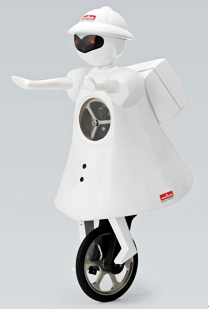
\includegraphics[height=5cm]{figures/murata_girl.jpg}
      \label{fig:murata}
    }
    \subfigure[Naveh's Model]{
      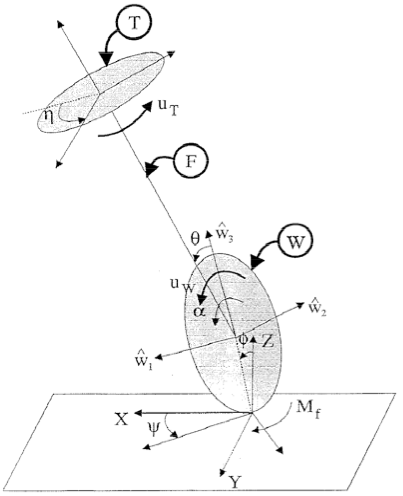
\includegraphics[height=5cm]{figures/naveh_unicycle.png}
      \label{fig:naveh_unicycle}
    }
    \subfigure[2D Problem]{
      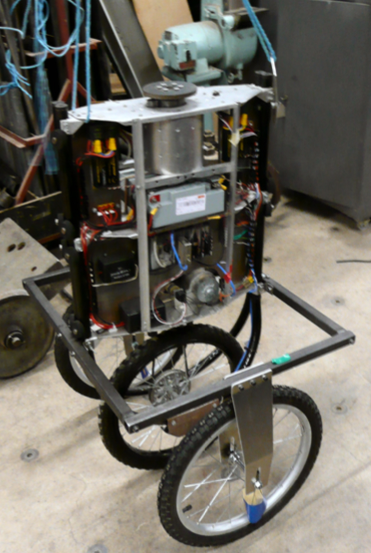
\includegraphics[height=5cm]{figures/forster_unicycle.png}
      \label{fig:forster_unicycle}
    }
    \subfigure[3D Problem]{
      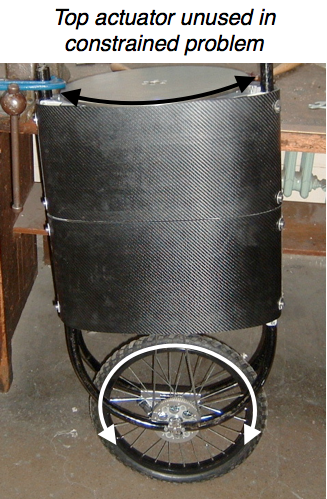
\includegraphics[height=5cm]{figures/3d_unicycle.png}
      \label{fig:3d_unicycle}
    }
    \end{center}
    \caption{Different balance problems}
    \label{fig:unicycles}
    \end{figure}

In 2004/2005 Mellors and Lamb \cite{ref:mellors,ref:lamb} built a robotic
unicycle, shown in Figure~\ref{fig:3d_unicycle}, intending to design a controller to balance it. However, they were
only able to complete the construction of the unicycle. In 2007/2008,
D'Souza-Mathew resumed work, replacing a wheel sensor and attempting to design
a controller. He simplified the problem by removing the ability to fall to the
side, reducing it to 2D dynamic control: the inverted pendulum (from
now on referred to as the 2D system). This is shown in
Figure~\ref{fig:forster_unicycle}. He was unable to balance the unicycle due to
hardware problems.

Next, in 2008/2009 Forster analysed the dynamics of both the 2D problem and
the unrestricted 3D unicycle\cite{ref:forster}. Again, hardware problems
prevented him from balancing the 2D system, and although he designed a
controller for the 3D unicycle, it was not even tested in simulation. Given
the simplicity of his approach compared to those of Vos and Naveh
\cite{ref:vos,ref:naveh}, it appears unlikely to work.

One thing all these approaches have in common is that their first step is a
series of simplifying assumptions about the dynamic system. They ignore the
non-linearities like motor dead-zones and wheel friction that are present in
any real-world system, and attempt to design a controller to stabilise the
idealised system. In many cases, this approach is very successful. However,
D'Souza-Mathew and Forster found that their model was invalid since the
unicycle's motor drive didn't react faster enough. Vos and Naveh had to use
complex, approximate techniques to model the unicycle.

An alternative ``intelligent'' approach to control involves learning the
dynamics of the system directly, instead of relying on assumptions and
mechanical analysis. Various methods for this have been used, but many require
prohibitively large amounts of data from the system. One method due to
Rasmussen and Deisenroth, known here as Reinforced Model Learnt Control
(RMLC), achieves unprecedented data efficiency, and has been successfully used
to stabilise a computer simulation of a 3D
unicycle\cite{ref:rasdei08,ref:rasdei11}.

In 2009/2010, McHutchon successfully applied RMLC to the 2D system
\cite{ref:mchutchon}. However, since he had to make significant changes to the
unicycle hardware and software to achieve this, he did not have time to
attempt to balance the 3D unicycle.

The principle objective of this project is to apply RMLC to the unrestricted
3D unicycle. This includes the solution of problems identified by McHutchon,
as well as other problems identified during the project.


\section{Reinforced Model Learnt Control}

The main technique in this project is Reinforced Model Learnt Control,
diagrammed in Figure~\ref{fig:rmlc_flowchart}. At its core, it assumes that
the system (in this case, the unicycle) can be modelled in discrete time as:
\[
  \boldsymbol{q}[n+1] = \boldsymbol{f}(\boldsymbol{q}[n],
  \boldsymbol{u}[n])
\]

In this equation, $\boldsymbol{q}[n]$ is the state of the system at time $n$,
and $\boldsymbol{u}[n]$ is control input at time $n$. In the case of the
unicycle, $\boldsymbol{q}$ consists of angles and angular velocities of the
components of the unicycle, and the position of the unicycle.
$\boldsymbol{u}$ consists of the commands sent to the wheel and flywheel
motors.

This function, $\boldsymbol{f}$, is modelled as a Gaussian Process (GP). By
using Gaussian Process Regression (GPR), we can estimate any continuous
function from sampled inputs and outputs. For a description of the mechanics
of GPR, refer to \cite{ref:gpml}. When the unicycle runs, we get
a series of states and control inputs that can be converted to samples of
$\boldsymbol{f}$, and this allows us to use GPR to estimate
$\boldsymbol{f}$ at any point. This estimated $\boldsymbol{f}$ is referred to
as the \textbf{dynamics model}.

By successively applying $\boldsymbol{f}$ to an initial distribution of
possible starting states, we can estimate, with confidence bounds, a
distribution of states over some finite horizon. This is referred to as
\textbf{simulation} of the system. Then, a \textbf{loss function} is applied
to the state distributions---this might find, for example, the expected
distance between the top of the unicycle and the upright position.  Summing
these losses over the horizon gives a numerical score that rates how well the
dynamics model believes a given controller will balance the unicycle. This
loss score penalises uncertainty as well as falling.

The gradient of the loss with respect to the controller parameters can be
calculated, and this allows standard gradient descent optimisation methods to
be used to find a locally optimal controller (for the estimated dynamics
model). This process is shown as the right-hand box, ``Simulation \&
Controller Optimisation'', in Figure~\ref{fig:rmlc_flowchart}, and is referred
to as \textbf{training} a controller.

Once a optimal controller has been trained on the simulated system, a
\textbf{rollout} is performed on the real system (``Real World Testing'' in
Figure~\ref{fig:rmlc_flowchart}). This generates a log of states and control
inputs, which can be converted into more samples of $\boldsymbol{f}$,
improving the quality of the dynamics model and allowing a better controller
to be trained. This process is repeated iteratively until the dynamics model
is sufficiently accurate that the trained controllers perform well on the real
system.

\begin{figure}[htbp]
  \begin{center}
    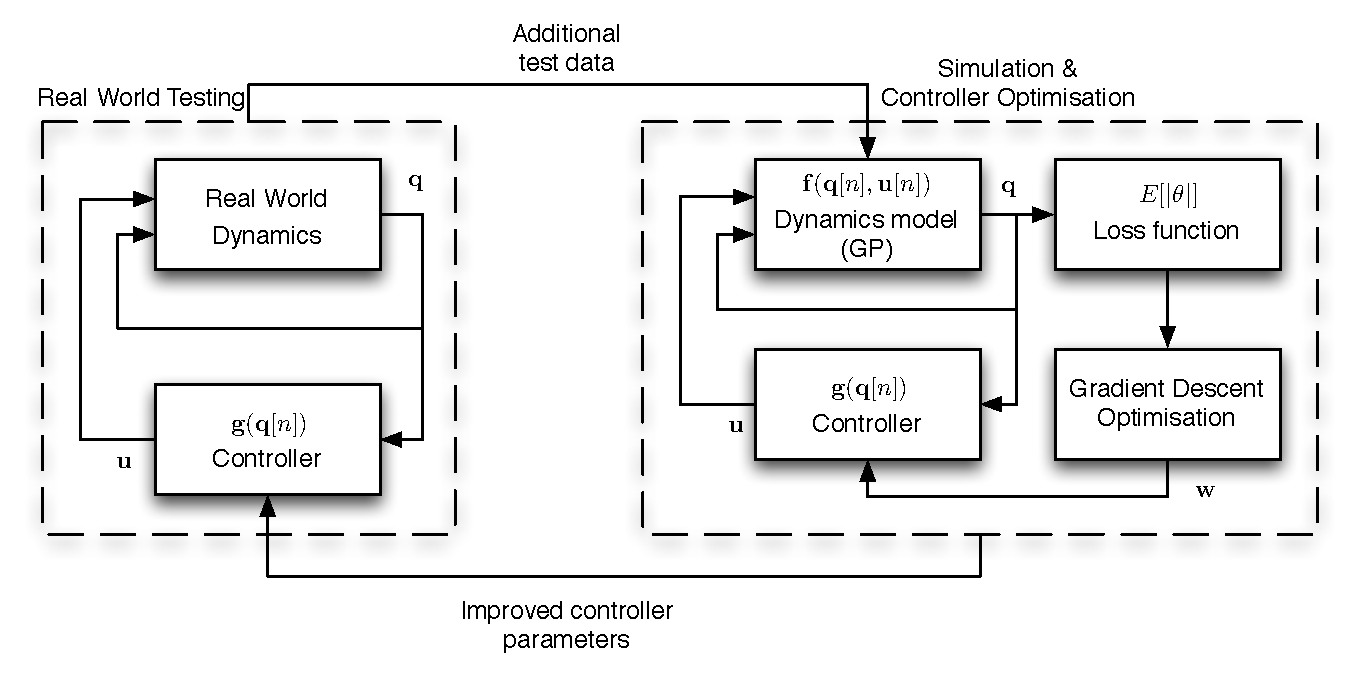
\includegraphics[width=14cm]{figures/GPRMLC.pdf}
    \end{center}
    \caption{Reinforced Model Learnt Control}
    \label{fig:rmlc_flowchart}
    \end{figure}

\section{Apparatus and Experimental Results}

\section{Results and Discussion}

\section{Conclusions}

\bibliography{iibproject}
\bibliographystyle{unsrt}

\pagebreak
\appendix

\section{Extra Stuff}

\end{document}
